\documentclass[adobefonts,11pt]{book}


\usepackage{ctex}
\usepackage{amsmath}


\usepackage{geometry}
\usepackage{makeidx}
\usepackage{paralist}
\usepackage[colorlinks=true]{hyperref}
\usepackage[format=hang,font=small,textfont=tt]{caption}

\usepackage{color}
\definecolor{pblue}{rgb}{0.13,0.13,1}
\definecolor{pgreen}{rgb}{0,0.5,0}
\definecolor{pred}{rgb}{0.9,0,0}
\definecolor{pgrey}{rgb}{0.46,0.45,0.48}



\usepackage{listings}
\lstset{% Global setting
	%language=XX,
	backgroundcolor=\color{white},
	basicstyle=\ttfamily,
	keywordstyle=\bfseries,
	commentstyle=\rmfamily\itshape,
	stringstyle=\color{pred}\ttfamily,
	flexiblecolumns,
	showspaces=false,
	showtabs=false,
	breaklines=true,
	showstringspaces=false,
	breakatwhitespace=true,
	tabsize=2,
	commentstyle=\color{pgreen}
	%numbers=left,
	%numberstyle=\footnotesize	
}

\lstset{% Global setting
	language=Fortran,
	basicstyle=\sffamily\small,
	keywordstyle=\bfseries,
	commentstyle=\rmfamily\itshape,
	stringstyle=\ttfamily,
	flexiblecolumns,
	%numbers=left,
	%numberstyle=\footnotesize	
}

\lstset{% Global setting
	language=Java,
	basicstyle=\ttfamily\small,
	keywordstyle=\bfseries\color{pblue},
	commentstyle=\ttfamily\slshape,
	stringstyle=\ttfamily\color{pblue},
	flexiblecolumns,
	xleftmargin=.5in,
	%numbers=left,
	%numberstyle=\footnotesize	
}

\usepackage{graphicx}




\setmainfont{Minion Pro}
\graphicspath{{../img/}}

\newenvironment{oopquote}
	{\begin{quote}\kaishu\zihao{-5}}
	{\end{quote}}


\makeindex

\title{面向对象笔记}
\author{theqiong.com}
\date{\today}


\bibliographystyle{plain}

\begin{document}

\maketitle
\tableofcontents
\listoftables
\listoffigures
\printindex

\part{Introduction}


\chapter{Overview}

\begin{oopquote}
结构化程序设计基于任务的层次划分,而面向对象的设计则基于数据对象的层次划分。
\end{oopquote}

面向对象思想\cite{oop}诞生于20世纪60年代,并且最早被应用于Simula语言中,到20世纪80年代才真正引起计算领域的普遍关注。

在应用面向对象编程技术来进行开发时,类用来代表一组相似的对象(例如整数、链表等),通过类的继承可以形成树状结构,每个类实例的存储空间和行为自动地被其派生类使用,而且同一个类的多个实例对象能够执行相同的行为。

类可以看作是用来保存与一个对象相关的行为的存储仓库,而且在实践中可以将类组织成一个单根树状结构,称为继承层次。

在对象之间传递的消息是对特定行为的请求,并且伴随着完成这项任务所需的参数。

\begin{enumerate}
\item 任何事物都是一个对象。
\item 通过互相联系的对象请求其他对象执行一定的行为来完成计算。
\item 对象之间通过发送和接收消息\footnote{消息(message)是指对特定行为的请求,并且伴随着完成这项任务所需的参数。}进行通信。
\item 每个对象都有自己的存储空间,用来存储其他对象。
\item 每个对象都是一个类的实例。
\end{enumerate}


从最细微的问题到最复杂的项目,我们时刻在面对“软件危机”,即我们通过计算机来解决复杂任务的难度几乎总是要超出我们的实际能力。

在众多针对“软件危机”的解决方案中,面向对象编程是最近提出的一种方法。

使用面向对象技术有利于构建复杂的软件体系结构,但是面向对象编程是一种新的思考问题的方法,它着重于面向对象对于计算的含义,以及如何构建信息才能把我们的意图与其他人和机器进行顺利的交流,它更加要求优秀的程序员的天赋、创新、勤奋、逻辑思维、构建和提取抽象的能力以及经验。

充分有效地利用面向对象原则需要人们以一种新的方式来观察世界,但是,简单地应用一种面向对象语言本身并不能使我们成为一名真正的面向对象开发者。

使用面向对象语言只是会简化面向对象解决方案的开发,这并不代表掌握了面向对象思想,而且使用面向对象语言也可以开发面向过程的程序。


在人造的计算机语言中,语言与思维之间的关系比其在自然语言中表现得还要显著,也就是说,选择哪种程序设计语言来考虑待解决的问题,会影响或改变算法的设计。

\section{FORTRAN}


下面以基因研究中的一个问题来证明计算机语言和问题解决方案之间的关系。

为了简化某一项分析DNA序列的任务,可以用一个由N个整数组成的矢量来表示DNA,其中N非常大(大约好几万)。我们的任务是判断DNA序列中是否包含重复的长度为M的序列片断,其中M为固定的数值常量(比如5或10)。


\begin{figure}[htbp]
\centering
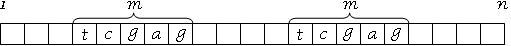
\includegraphics[scale=0.7]{dna-vector.png}
\caption{由N个整数组成的矢量来表示的DNA序列}
\label{fig:dna-vector}
\end{figure}

使用FORTRAN语言编写的解决这个问题的计算机程序如下:

\begin{lstlisting}[language=Fortran]
		DO 10 I = 1,N-M
		DO 10 J = 1,N-M
		FOUND = .TRUE
		DO 20 K = 1,M
20	IF X[I+K-1] .NE. X[J+K-1] THEN FOUND = .FALSE
		IF FOUND THEN ...
10	COUTINUE
\end{lstlisting}

\section{APL}


如果使用APL语言来编写上述这个问题的解决方案,需要重新考虑这个问题。例如,可以把数据重新安排在一个N行M列的矩阵中,而不是前面所使用的由N个元素组成的矢量。

\begin{figure}[htbp]
\centering
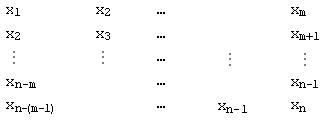
\includegraphics[scale=0.7]{dna-apl.png}
\caption{使用N行M列的矩阵表示DNA序列}
\label{fig:dna-apl}
\end{figure}

把矩阵按行排序(即把一行看作一个单元,在排序过程中移动整行)。如果有任何序列片断被重复,那么在排序后的矩阵中相邻的两行就会有相同的数值。

\begin{table}[htb]
\centering
\begin{tabular}{cccccc}
.&	.&	.&.	&.	&.	\\
T	&G	&G	&A	&C	&C\\
T	&G	&G	&A	&C	&C\\
.&	.&.	&.	&.	&.	\\
\end{tabular}
\end{table}


检查如何满足这项条件很容易。在这里,APL程序之所以快与APL语言本身无关,而是与算法有关。简单的讲,FORTRAN程序使用了一个$O(M\times N^2)$的算法,而APL程序使用的排序方案需要大约$O(M\times N\log N)$次操作。


上述示例的目的并不是说明APL语言在任何情况下,都比FORTRAN语言更有效,而是指APL程序员很自然地被引导发现一种完全不同的解决方式。

虽然使用APL语言很难写循环,而排序却很简单——作为语言组成部分,排序被定义为内部操作符。

在APL语言中,排序运算很容易表达,APL程序员倾向于寻找关于它的创新性应用,这也就说明了解决问题的编程语言是如何引导程序员采用不同的思维方式来看待问题的。

表达思想的语言可以影响或引导思维,这一点在程序设计语言方面得到了很好的体现,因此Spair-Whorf假说认为存在这样一种情况:

\begin{quote}
\texttt{一个生活在某种特定语言环境下的人可能产生或者表达一些想法,这些想法无论如何也无法被生活在另外一种语言环境下的人所翻译和理解。}
\end{quote}

根据Spair-Whorf假说提倡者的观点,这种现象可能发生的情况是在后者的语言中没有对应的词汇或者缺少相关的概念来表达前者的想法。


\section{Turing Machine}

将人类语言产生上述这种现象的可能性与计算机科学中几乎直接对应的计算机语言产生这种现象的可能性相比较是一件有趣的事情,因此逻辑学家Alonzo Church发表了如下的丘奇猜想(Church's Conjecture)。


\begin{quote}
\emph{任何一种具有明确步骤的计算都可以通过图灵机来实现。}
\end{quote}





图灵机是一种可不受存储容量限制的假想计算机,但是图灵机本身是一种极其简单的装置,不需要有很多特性的某种语言来模拟这个装置。

如果我们接受丘奇猜想,那么任何可以模仿图灵机的语言都足以运算任何可实现的算法。为了解决这个问题,首先需要寻找能够生成所期待结果的图灵机。通过丘奇猜想可以知道这种图灵机一定存在,然后用我们所擅长的语言来模拟图灵机的运行。这样关于编程语言相对“能力”的讨论——如果我们把能力理解为“解决问题的能力”——是毫无意义的,而且我们也就陷入了Alan Perlis所提出的“图灵机泥潭”中,这种讨论既无意义又难以摆脱。



需要注意的是,丘奇猜想在某种意义上几乎与Spair-Whorf假说完全对立。


\begin{compactitem}
\item \texttt{丘奇猜想认为在基本方法上,所有的编程语言都是一样的。或者说,一种语言能够表达的想法,在理论上,用另一种语言也能表达。}
\item \texttt{Spair-Whorf假说则认为,存在这样一种可能,某些想法能用一种语言表达,却不能用另外一种语言表达。}
\end{compactitem}

由于无法对“明确的步骤”进行严格的限定,因此天生注定丘奇猜想没有被证实,也无法被证实。不过,至今还没有发现它的反例,似乎可以证明丘奇猜想的可靠性。


人们后来对自然语言提出了一种“图灵机-等价”理论,意思是说,只要通过充分的工作,任何想法都可以用任何语言来表达。

例如,一个一直生活在热带的人无法直觉地用自己的语言对不同类型或用途的雪进行分类,也无法判断雪域的范围,但是只要通过一定时间的培训,就一定能够掌握这种技能。

同样,面向对象技术也不能提供任何新的计算能力,使得原来通过其他方法在理论上无法解决的问题得到解决,但是面向对象技术确实提供了一种方式,使得解决问题更加容易和自然,而且这种方式有效地改善了大型软件项目的管理。


无论是计算机语言还是自然语言,语言只能引导思维,而不能阻止思维。面向对象编程不仅仅是在编程语言中加入一些新的特征,更重要的是,它是用来分析处理问题和开发计算机程序解决方案的一种崭新的思考方式。

可以肯定地说,一个由具有共同兴趣的个体组成的群体,倾向于发展他们自己的特殊词汇,一旦这些词汇形成,它们就会影响这些人的思维方式,而对于群体以外的人,这种方式很难理解,这本身就是一个OOP的实例。

既然面向对象思想在一定的原则下不需要面向对象语言就可以使用,那么面向对象术语的使用就能够帮助用户以一种对于没有OOP术语的人来说也能理解的方式去思考问题。


\chapter{Real World}

下面首先考虑一下我们如何处理现实世界的情况,然后再去考虑在使用计算机解决问题时如何应用这种技术模式。

假设有一位名叫Chris的人想送花给他的一位叫Robin的朋友,Robin生活在另外一个城市。因为距离太远,Chris不能亲自把花送给他的朋友。不过,可以通过别的办法来完成。Chris来到附近的一家花店,这家花店由一个名叫Fred的花商经营。Chris把打算送给Robin的花的种类和Robin的地址告诉给Fred。这样Chris就可以确信他的花可以方便地送到他的朋友那里了。

\begin{figure}[htbp]
\centering
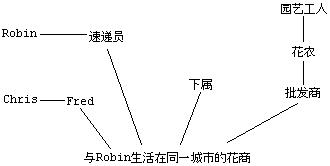
\includegraphics[scale=0.65]{flower.png}
\caption{现实世界中的实例}
\label{fig:flower}
\end{figure}

这里解决问题的方法就是找到一个合适的代理(也就是Fred),并且把自己的要求告诉他。代理有责任完成这些要求,Fred会选择某种方式——一种算法或一系列操作——来完成这项任务。Chris没有必要了解Fred使用什么方法来完成任务。实际上,使用代理的人通常不想了解完成任务的细节,这些细节一般都是隐蔽的。

通过调查可以发现,Fred向一位与Robin生活在同一城市的花商传递了一条信息,然后,那名花商可能会让一名下属来安排这件事。接着花和另外一条消息将交给一个速递员。这样依次进行下去。此时我们又会发现,与Robin生活在同一城市的那个花商一直都从花卉批发商那里购进花。同样地,花卉批发商又与花农交易,而花农则要管理园艺工人。

由此,我们得到关于通过面向对象思想解决问题的初步结论:解决问题需要很多其他个体的帮助。没有这些个体的帮助,问题难以解决。简单概括如下:

\begin{quote}
\emph{一个面向对象程序可以由一个团体(集合)组织而成,这个团体由一组互相作用但又松散连接的叫做“对象”的代理组成。每一个对象都扮演一个角色,对特定的任务负责,并且为团体中的其他成员提供特定的服务或者执行特定的行为。}
\end{quote}

设计一个面向对象程序就像组织一个团体,团体中的每个成员都被赋予一定的责任,这样程序功能的实现就来自其中每个对象的努力及它们之间的相互协作。

\section{Message}

开始,Chris向花商Fred提出要求,此项要求导致了另外一项要求,然后又继续导致更多的要求,直到花最终送到Chris的朋友Robin手中。

通过这一系列的连锁反应,Chris的要求最终被实现了,而且由此可以看到,团体的成员通过传递要求来相互协作。

下面提出的通过面向对象思想解决问题的原则是确定传递工具来指示下一步行为。

\begin{quote}
\textbf{在面向对象编程中,行为的启动是通过将“消息”传递给对此行为负责的代理(对象)来完成的。}

\textbf{消息对行为的要求进行编码,并且伴随着执行要求所需的附加信息(参数)来一起传递。“接收器”就是接收消息的对象。}

\textbf{如果接收器接收到了消息,那么同时它也接受了消息所包含的行为和责任,然后接收器响应消息,并执行相应的“方法”以实现要求。}
\end{quote}

与消息传递相关的是信息隐蔽原则——提出要求的客户不需要了解实现该要求的具体方式,还有另外一条原则——我们所知道的所有人都是隐藏在消息传递过程中的。客户如果要完成一项任务,首先的想法就是寻找能够执行这项任务的人。


面向对象编程的一个重要部分就是可复用组件的开发。使用可复用组件的第一步,也是非常重要的一步,就是程序员能够接受、信任他人编写的软件。在实际的计算机解决方案中,最终是通过对象的相互作用来完成计算的。

在传统的语言中,信息隐藏(information hiding)也是编程的一个重要方面。虽然根据要求两者都会运行一系列预定义的步骤,但是它们也有两点截然不同的地方。

\begin{description}
\item[首先] 每一条消息都与一个指定的接收器相对应,接收器就是接收消息的对象。过程调用却没有指定的接收器。
\item[其次] 消息的解释(即用于响应消息的方式)由接收器来决定,并且随着接收器的不同而不同。
\end{description}

例如,Chris给他的一位名叫Elizabeth的朋友发了一条消息,她接收到消息之后,立即采取了相应的行动(即把花送给了他们共同的朋友Robin)。但是,Elizabeth完成要求的方法和Fred完成相同要求的方法是完全不同的。

如果Chris让牙医Kenneth将花送给Robin,而Kenneth可能没有办法解决这一问题。如果他完全理解了这个要求,则有可能向Chris返回一个信息来说明错误。

从上述可以得出,消息传递与过程调用有如下的区别:

\begin{quote}
\texttt{消息传递有一个指定的接收器,解释——选择响应消息的方法——可能因接收器的不同而不同。}
\end{quote}

通常,人们在程序运行之前不会知道任何消息的接收器,也不会知道调用了哪些方法。

一般情况下,消息(函数或过程名称)和响应消息的代码段(方法)之间是后期绑定的关系。与之对应的是,传统过程调用中名称与代码段之间的早期(编译时或链接时)绑定关系。

\section{Responsibility}


面向对象编程的一个基本概念就是用责任来描述行为。例如,Chris对行为的要求仅仅表明他所期望的结果(把花送给Robin)。Fred可以任意选择使用的方法来实现所期待的目标,并且在此过程中不会受到Chris的干扰。

通过用责任来讨论问题,提高了问题抽象的水平,使得对象之间更加独立,这正是解决复杂问题的关键。通常用协议来描述与一个对象相关的所有责任的集合。

传统程序的执行通常是通过对数据结构进行操作——例如,改变数组或记录中的域。与此相反的是,面向对象程序则要求数据结构(即对象)提供服务。


从传统的、结构化数据的角度来观察软件与从面向对象的角度来观察软件之间的区别,可以得到下面的结论:

\begin{quote}
\emph{不要问你能为数据结构做什么}

\emph{要问数据结构能为你做什么}
\end{quote}

\section{Class}

在上述示例中,Chris对Fred提出送花给Robin的要求之后,他大致上可以认定这个事件会发生在Fred的花店里。Chris做出这样的假定是基于以往同其他花商打交道的经验,因此Chris认为Fred作为这一类别中的一个实例,应该适用普遍的模式。

这里。我们可以用花商来代表所有花商中的一个类别(或者是类),从而可以把这些概念总结成面向对象编程的另外一个原则:

\begin{quote}
\emph{所有对象都是类的实例。}

\emph{由类的接收器来决定在响应消息时调用的方法。}

\emph{一个特定类的所有对象使用相同的方法来响应相似的消息。}
\end{quote}

对象是对状态(数据值)和行为(操作)的封装,因此对象和专用计算机有很多相似之处。

\begin{compactitem}
\item 对象的行为由对象类来规定。
\item 每个对象都是某个类的一个实例。
\item 同一个类的所有实例都以相似的方式(即调用同一方法)来响应相似的要求。
\end{compactitem}





对象通过调用方法表现其行为(类似于执行一个过程),并以此来响应消息。对消息(即所使用的特定的方法)的解释由对象决定,并且随着对象类的不同而不同。



\section{Inheritance}

Chris还有Fred更多的信息——这不仅是因为他是一个花商,更是因为他是一个店主。例如,Chris知道钱的转移是这项交易的一部分,同时作为付款的凭证,Fred交给Chris一张收据,而这些行为同样也会发生在食品商、文具商和其他店主身上。由此可知,花商这个类别是店主类别的一个特殊类别。Chris知道,关于店主的一切对于花商也同样适用,于是这也适用于Fred。

下面将讨论Chris是如何组织关于Fred的信息的,我们可以通过分类层次来考虑。Fred是一个花商,而花商又是店主的一种特殊形式。进一步讲,店主是一个人。而Chris知道所有关于人的一切也同样适用于Fred,尽管这些信息没有直接与他发生联系。


一般类别的信息也适用于特殊类别,这样的原则称为继承。

通常情况下,可以利用一种交错的图像技术来说明继承关系(尤其是当很多个体有不同的归属时),通过继承技术可以把类组成树状层次结构。其中,继承结构中的比较抽象的类位于树的顶端,比较具体的个体位于树的底部。

\begin{quote}
\texttt{类可以组织成一个有层次的继承树结构。}

\texttt{子类继承层次树中更高一层的父类的属性和行为。}

\texttt{抽象父类不能有具体实例,只能用来产生子类。}
\end{quote}


继承的引入使得树中较低层次的类可以存取和使用与树中较高层次的类相关的数据和行为。


\section{Override}

为了解决类的层次结构中平行类的相关问题,需要寻找一种技术,能够处理一般规则以外的特例。

我们可以通过在子类中发布一条信息来解决此问题,这条信息可以改写(override)从父类继承的信息。通常,给子类中某一方法取一个与父类中某一方法相同的名称,再结合寻找方法的规则(当响应特定信息时)来实现这个目的。

\textbf{接收器类搜索并执行相应的方法以响应给定的消息。如果没有找到匹配的方法,搜索就会传导到此类的父类。搜索会在父类链上一直进行下去,直到找到匹配的方法,或者直到父类链结束。}

\begin{compactitem}
\item \textbf{如果是前一种情况,就会执行方法;}
\item \textbf{对于后一种情况,会产生错误信息。}
\end{compactitem}

\textbf{如果能在更高类层次找到相同名称的方法,所执行的方法就称为\textcolor{blue}{改写}了继承的行为。}

虽然编译器在运行时不能确定调用哪个方法,但是许多面向编程语言能够确定是否有合适的方法以供调用,并且能够产生错误信息作为编译时错误诊断,而不是运行时信息。

不同的对象都会对类的消息做出相应的反应,但执行的方法却不同,这也就是多态(polymorphism)的一种表现。

例如,Elizabeth和Fred都会对Chris的消息作出反应,只是执行的方法不同,而且Chris不了解也不需要确切地了解Fred使用的方法,从而也对信息进行了有效的隐藏。

\chapter{Metaphor}



计算机执行程序的行为的模型是一个过程状态或者鸽子窝模型,或者说,计算机是一个数据管理员,跟随着一些指令模式,在存储器中从不同的槽(内存地址)中取出数值,用某种方式对它们进行转换,再将结果推入到另外的槽中。检查槽中的数值就可以确定机器的状态或者计算的结果。

虽然这个模型与实际计算机内部的工作流程大致吻合,但对于我们理解如何使用计算机来解决问题,却没有多少帮助,而且这也不是我们大多数人解决问题的方式。

在面向对象框架中,用户几乎不提内存地址、变量、赋值或者任何传统编程术语,只是使用对象、消息和某种行为的责任。

在面向对象编程思想中,用户拥有的是一组行为规范的对象,各个对象之间通过礼貌地交互来实现各自的愿望。


在很多方面,把编程比作创建“域”的观点和一种称为“离散事件驱动模拟”的计算机模拟很相似。简而言之,在离散事件驱动模拟过程中,用户为不同的模拟元素创建其计算机模型,通过模型来描述元素之间如何相互作用,并使它们运作起来,这几乎等同于通常的面向对象程序。

在通常的面向对象程序中,用户需要描述域中的不同实体代表什么、它们如何相互作用以及如何使它们最终运作起来,因此我们可以得到下面这样的结论。

\begin{quote}
\textbf{在面向对象编程中,计算就是模拟。}
\end{quote}

面向对象编程把程序看成是一个集合,这个集合由称为对象的松散连接的代理组成。

\begin{compactitem}
\item 每个对象都对特定的任务负责。
\item 通过对象的相互作用进行计算。
\end{compactitem}

从某种程度上说,编程就是一个对模型域的模拟。通过类和模拟的概念,初学者可以更容易地理解隐喻(metaphor)。

隐喻有利于面向对象技术的应用,但是通常它却很容易被忽略。例如,当用户根据对象的行为和责任思考问题时,可以为用户带来很多的关于日常经验的直觉、思想和理解力。

如果把问题想象成鸽子窝、邮箱或者包含数值的槽时,用户几乎不需要什么背景知识就可以深入了解问题并对其结构化,这些都是隐喻的强大的解释力量的反映。

不同于以往的编程方法,使用面向对象编程思想分析问题和编写程序解决问题时,为开发者提供了更大的构件,开发者通过迅速地用它们组装自己的软件就可以解决问题,这一方面可以类比Lego玩具提供的各种组件。

通过减少软件组件之间的相关性,面向对象编程可以实现可复用软件系统的开发。

可复用的组件与软件应用的其他部分是隔离的,从而可以作为独立的单元来创建和测试,而且可复用的软件组件允许用户在更高的抽象层次上处理问题,这样就可以简单地通过能被对象所理解的消息和对象需要执行的任务来定义和操作对象,而不必考虑执行细节。

当然,对象不可能总是通过礼貌地请求另一个对象执行某种行为来响应消息。如果这样,结果会形成一个无限的请求循环,就像两个绅士都礼貌地等待另一位先进门,或者像一个使用纸上签字的官僚机构,每一个人都把所有的待签纸传给组织中的另外的人。

在某种程度上,至少有几个对象,除了传递请求给其他代理之外,还执行一定的工作。根据所使用的面向对象语言的不同,这项工作的完成情况也不同。

\begin{compactitem}
\item 面向对象/命令的混合语言(如C++语言、Object Pascal语言和Objective-C语言)通过基础(非面向对象)语言编写的方法来完成。

\item 更加纯粹的面向对象语言(例如Smalltalk或者Java)是通过语言基本体系结构所提供的“原始的”或者“固有的”运算指令来完成。
\end{compactitem}

另外,Peter Wegner提出了区别基于对象语言和面向对象语言的不同之处的方法,基于对象语言只支持抽象(如Ada),而面向对象语言还必须支持继承。

\begin{quote}
\texttt{Apple Object Pascal语言最初是由Larry Tesler定义的,Borland Pascal语言最终演化成了Delphi语言。Objective-C语言的创建者是Brad Cox,在它作为C语言的扩展语言产生的同时,C++语言也开发完成,Smalltalk语言也有其公共流行版本Squeak。}
\end{quote}

\chapter{Abstraction}

在打开一本地图册时,首先会看到一张世界地图,而且其中只会显示某些最重要的特征,例如各种山脉、河流和其他一些非常大的建筑物,一些细小的特征都被忽略了。

随后的地图会描绘出一些小的地理区域(通常还有更多的细节),例如:

\begin{compactitem}
\item 一个洲的地图可能包括政治边界和一些主要的城市;
\item 一张关于更小区域的地图(例如一个国家)可能包括城市、乡村和更小的地理特征,比如某个山脉的名称;
\item 一张大城市的地图可能包括出入城市的主要道路;
\item 比城市更小的区域地图甚至可能标注出每一座建筑。
\end{compactitem}

在每一级别水平上都会包括某些特定的信息,而故意忽略了某些其他的信息。当以更高级别的抽象来看待一件制品时,没有什么方法能够描述它的细节。

即使能够描述出这些细节(比如用极小的字),人们也无法吸收或处理如此大量的信息,因此一些细节就这样简单地被忽略了。

通常,人们只使用几种简单的工具去创建、理解和管理复杂的系统,其中抽象就是最重要的技术之一。

\begin{quote}
\texttt{抽象(abstraction)是指对于一个过程或者一件物品的某些细节的有目的的隐藏,以便把其他方面、细节或者结构表达得更加清楚。或者说,抽象就是为了强调指定的特征而有目的地压缩细节。}
\end{quote}



用户通过抽象可以建立起针对实际系统的不同层次的模型,因此抽象通常与组件划分相联系。

在形成抽象或模型时,需要有意识地避免理解很多细节,并且集中精力在几个主要特征上面,因此经常使用另外一个术语来描述这样的行为:信息隐藏。

\begin{quote}
\texttt{信息隐藏描述了部分抽象,通过它就可以有意地忽略某些特征,以便于能够集中强调其他特征。}
\end{quote}

抽象产生的组件封装(encapsulate)了某些主要特征,并通过简单和固定的接口(interface)与其他组件进行相互。

\section{Abstraction Level}


在一个典型的面向对象程序中,有很多抽象层次。

\begin{compactitem}
\item 更高层次的抽象体现了面向对象程序的特征。
\item 在最高层次的抽象层次上,程序被看作是一个由很多对象组成的“团体”。
\end{compactitem}


\begin{figure}[htbp]
\centering
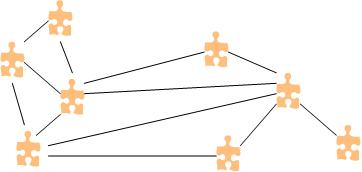
\includegraphics[scale=0.6]{abstract-level.png}
\caption{抽象层次}
\label{fig:abstract-level}
\end{figure}


在面向对象开发中,团体这个概念有两种不同的形式,而且信息隐藏和抽象等面向对象思想对这两种形式都适用。

\begin{compactitem}
\item 程序员团体

在现实世界中,为了完成应用程序,程序员之间必须互相合作。
\item 程序员创建的对象团体

在虚拟世界里,对象之间必须互相合作来实现共同目标。
\end{compactitem}



团体中的每一个对象都为组织中的其他成员提供服务,在最高级别的抽象层次上需要强调的最重要的特征就是交流和合作的通道,以及成员之间相互合作的方式。

下一个级别的抽象不会在所有的面向对象程序中出现,也不被所有的面向对象语言所支持。但是,很多语言都允许一组对象一起工作,形成一个单元(unit)。

关于这个思想的实例有Java语言中的包(packages)、C++语言中的名称空间(name spaces)和Delphi语言中的单元(units),这样就允许某些特定的名称暴露在单元以外,其他的特征则隐藏在单元内部。

\begin{quote}
\texttt{实际上,单元的概念继承了C和Modula等语言中的模块(module)思想,面向对象编程思想应归功于早期的模块研究。}
\end{quote}


下面两个级别的抽象是用来处理两个独立对象之间的交互。例如,我们常说的是一个对象能够为其他对象提供服务,这种直觉的建立来自于对客户和服务器之间通信的描述。

这里的服务器只是表示提供服务的对象,而且这两个层次的抽象涉及了对这种关系的两种视角,一种来自于客户端,一种来自于服务器端。


在一个优秀的面向对象设计中,我们可以描述和讨论服务器所提供的服务,而无需提及客户在使用这些服务时可能执行的任何行为。

下面可以把关于信息隐藏和抽象的表述想象成一个描述了数据结构(如堆栈)所提供的服务的广告牌。


\begin{figure}[htbp]
\centering
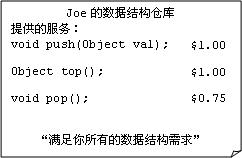
\includegraphics[scale=0.6]{ad-board.png}
\caption{广告牌}
\label{fig:ad-board}
\end{figure}

高级别的抽象通常用接口来表示,实际上接口是一个与类相似的结构,它定义了行为,但不描述如何来实现这些行为。

\begin{lstlisting}[language=Java]
interface Stack{
	public void push(Object val);
	public Object top() throws EmptyStackException;
	public void pop() throws EmptyStackException;
}
\end{lstlisting}


下一抽象层次查看同一边界,但却不同于服务器端。这里的抽象层次需要考虑抽象行为的具体实现。例如,有很多数据结构可以用来满足堆栈的要求,这样的抽象层次主要关注服务的具体实现方式。

\begin{lstlisting}[language=Java]
public class LinkedList implements Stack ...{
	public void pop()	throws EmptyStackException{...}
	...
}
\end{lstlisting}


在抽象的最底层需要单独考虑一项独立的任务(即一个方法),因此这一层次的抽象主要关注的是执行这一活动所需操作的精确顺序。例如,我们可能需要研究用来移走放入堆栈里的最近元素的操作。

\begin{lstlisting}[language=Java]
public class LinkedList implements Stack ...{
	...
	public void pop() throws EmptyStackException{
		if(IsEmpty())
			throw new EmptyStackException();
		removeFirst(); //delete first element of list
	}
	...	
}
\end{lstlisting}

在软件的开发过程中,每一个抽象层次在某些方面都很重要。实际上,程序员需要在各种抽象层次之间迅速地移动,也就要求在每一个抽象层次上执行相应的面向对象的分析。

在软件开发的早期,一个关键的问题就是如何确定正确的抽象级别,通常出现的错误是在低层次的抽象级别上反复思考,担心各种关键组件的实现细节,而不是努力地思考如何实现高级别的抽象来促进有关问题之间的完全分离。

在软件开发过程中的任何时刻,程序员(或开发一个比较大的项目的设计小组)都必须进行缜密的思考,才能确定正确的抽象级别。

对于特定问题,人们通常不愿忽略或者放弃很多的细节,但是实际上不能过多地关注细节,否则一些重要的问题就会被掩盖。


\section{Abstraction Pattern}

抽象可以用来帮助理解复杂的系统,从而反映出系统某些真实的方面,或者它可能只是一种思维的抽象,用来帮助我们理解真正的问题。

在某种程度上,抽象是系统结构的版图。

抽象的思想可以进一步划分为不同的形式,通常的技术是将一个层次划分成各种组成部分。例如,当我们描述汽车是由发动机、传动装置、车体和车轮组成时,所使用的正是这个方法。

下一个理解层次是通过依次检查每一个组成部分来实现,这不过是分而治之(divide and conquer,分治法)的一个体现。

\begin{figure}[htbp]
\centering
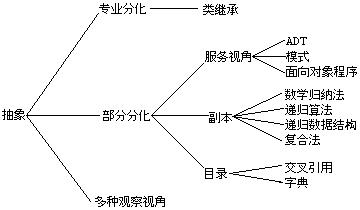
\includegraphics[scale=0.6]{abstract-pattern.png}
\caption{抽象的其他形式}
\label{fig:abstract-pattern}
\end{figure}

有时候我们使用不同类型的抽象,因此另外一种形式就是特化分层思想。

例如,对于汽车的理解就可以部分基于以下知识。首先,它是一个有轮子的车辆,其次,它是一种交通运输工具。

当我们还了解其他一些关于有轮车辆的知识后,这些知识既适用于汽车,也适用于自行车。如果还了解其他各种不同的运输工具,这些知识也可以同样地适用于驮马,也适用于自行车。

面向对象编程语言广泛地使用特化分层的抽象形式。

\begin{figure}[htbp]
\centering
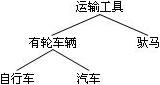
\includegraphics[scale=0.6]{abstract-example.png}
\caption{特化分层}
\label{fig:abstract-example}
\end{figure}

部分分化和专业分化的思想代表了在面向对象编程中使用的两种最重要的抽象形式,即通常所说的“是抽象”和“有抽象”。

\begin{description}
\item[是抽象]

专业分化是指“是抽象”,例如自行车“是有轮车辆”,它“又是运输工具”。

\item[有抽象]

部分分化就是“有抽象”,例如汽车“有发动机”。
\end{description}

在实际的计算机程序设计过程中,“是抽象”和“有抽象”会与特定编程语言的特征联系在一起。

人们最常使用的用来帮助理解复杂系统的技术就是把抽象和分化成的各种组件结合起来。

我们对汽车的描述就是一个这样的例子,理解下一个层次需要通过对每一个组成部分进行更精细的细节分析来实现。例如,对汽车发动机更精细一些的描述,就是把它看作圆柱体的组合,每一部分都能将燃料的爆炸转变成垂直方向的运动,并通过曲轴将圆柱体的上下运动转换成旋转运动。

另外一个例子是关于如何组织人体运动的信息。在某一层次上,我们只关系各种组织,把人体看作是由骨骼(保持刚性)、肌肉(产生运动)、眼镜和耳朵(产生感觉)、神经系统(传递信息)和皮肤(把各个部分连接起来)组成的。在下一个抽象层次上,我们可能会考虑肌肉是如何工作的,并且会考虑一些比如细胞结构和化学作用的问题,而化学作用又是由分子结构决定的。为了了解分子,又得把分子继续分解为原子。

任何解释都必须基于正确的抽象层次来阐述,因此如果试图以原子层次的细节来解释一个人是如何行走的,将会是极其困难的。


\section{Encapsulation}


创建一个大系统的关键步骤就是将其分成合理的组成部分。

实际上,不管是编写软件还是建造汽车,通过将整体的大的系统进行合理的划分,就可以分配人员基本独立地进行各部分的工作。



封装的基础是内部视角和外部视角之间有着严格的区分,因此制造发动机的小组成员对传动装置只需要有一个抽象的(也就是外部的)理解,而制造传动装置的小组成员则需要对传动装置具备详细的内部理解。

封装允许用户考虑实现互换的可能性,当把一个系统划分为几个部分时,理想的目标就是将各个部分之间的相互作用减少到最少。例如,通过封装发动机的行为可以与传动装置隔离,从而可以把一种类型的发动机转换成另外的类型,不会影响系统其他部分的运行。

为了将这些思想应用于软件系统,用户需要一种方式来讨论软件组件执行的任务,而且这种方式要和组件满足责任的方式区别开来。


\section{Interface}

在软件系统中,使用接口和实现这两个术语来描述一项任务包含哪些内容和如何实现任务,以及外部视角和内部视角之间的区别。

\begin{compactitem}
\item 接口描述系统被设计用来做什么,这是抽象使用者必须理解的思想。
\item 接口并没有说明所分配的任务应如何执行。
\item 接口通过与完成抽象的实现相匹配来使系统正常工作。
\end{compactitem}

在汽车工业中,发动机的设计者会与传动装置的接口相联系,而传动装置的设计者必须实现这些接口。

同样地,开发复杂的计算机软件系统的一个重要步骤就是将一项任务分成几个部分,这些部分可以由小组的不同成员来开发。其中,每一个部分都有两个方面:接口显示给外部世界,而实现用来完成接口的要求。

接口和实现的分离不但使得在较高层次上理解一项设计更加容易(因为接口的描述比任何特定实现的描述都简单得多),而且使软件组件的互换性成为可能(因为可以使用任何实现,只要它能够满足接口规范)。

\begin{quote}
\textsl{当一个系统中组件的数量越来越多的时候,以“目录”的方式来组织它们通常是很有效的。}
\end{quote}

在日常生活中我们要使用很多不同形式的目录。例如,电话号码簿、字典或搜索引擎等。类似地,在软件中也使用各种各样的目录,一份关于系统中所有类的简单列表就是一个这方面的例子。

另外一个目录的例子就是由类所定义的所有方法组成的清单,例如Java标准库的类参考手册就是一个非常有用的目录。

\begin{quote}
\textsl{目录为用户提供了一种机制,使用户可以从一个范围很大的集合中迅速地定位到某一特定的位置(可以是类、对象或者方法)。}
\end{quote}


接口描述了软件组件所提供的服务,但是不必描述完成服务所使用的技术,这个思想是理解和处理复杂软件系统的核心手段。例如,在上述关于送花的实例中,强调的也是这种抽象,而且这个实例的最后结果是有很多人都参与了送花的过程,并且在每个流程都各司其职。

\begin{figure}[htbp]
\centering
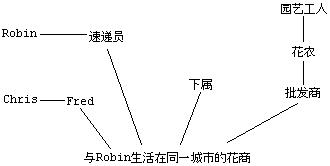
\includegraphics[scale=0.6]{interface-service.png}
\caption{服务视角}
\label{fig:interface-service}
\end{figure}


团体中的每个成员为这个团体中的其他人提供服务,没有一个成员能够自己独立地解决问题,只有通过互相协作,才能实现所期待的结果。




\section{Compounding}


复合法是另外一种从独立的部分创建复杂结构的强大技术。这一思想从少量几个基本的形式开始,然后增加一些规则,将各个形式结合起来创建新的形式。


\subsection{Regular Expression}


复合法的主要原则是允许合并机制,既可以作用于新形式也可以用在原来的基本形式上。例如,正则表达式(regular expression)就充分地说明了复合法技术。

正则表达式是描述一系列数值的简单技术,它的描述是从确认基础的字符表开始的。

以字符a、b、c和d为例进行说明,任何单独字符的例子都是一个正则表达式,然后我们可以增加一条规则,即由两个正则表达式组成的复合结构也是一个正则表达式。

\begin{lstlisting}[language=bash]
abaccaba
\end{lstlisting}

通过反复地应用复合法规则,就可以发现任何有限的由字符组成的字符串都是正则表达式。



下一个合并规则是说两个正则表达式的可替换形式(用竖线“|”来表示)是一个正则表达式。正则表达式遵循这样的运算规则,复合运算优先于可替换运算规则,因此下面的模式代表一系列由三个字母组成的值,由ab开始,并以a、c或者d结束。

\begin{lstlisting}[language=bash]
aba|abc|abd
\end{lstlisting}

如果可以用括号来表示分组,就还可以表示成下面的形式:

\begin{lstlisting}[language=bash]
ab(a|c|d)
\end{lstlisting}


最后,符号“*”(通常称为星号)用来表示“0或者多个重复”的概念,把这些规则结合起来就可以描述非常复杂的字母组合。

例如,下面一系列字符值的描述是以a或者b的循环紧接着一个c来开始,或者是以dd两个字母序列开始,然后是字母a。

\begin{lstlisting}[language=bash]
(((a|b)*c)|dd)a
\end{lstlisting}

\subsection{Type System}


\begin{quote}
\textbf{复合法的思想也是类型系统的基础。}
\end{quote}

类型系统始于原始类型(例如整数类型和布尔类型),类的思想允许用户创建新的类型,这些新的类型可以包含从前一类型构建出的数据字段。

这里的前一类型可能是原始类型,也可能是用户自定义的数据类型。既然可以以先前所定义的类为基础来创建类,那么就可以逐渐地构建出非常复杂的系统。


\begin{lstlisting}[language=Java]
class Box{ // a box is a new data type
	...
	private int value; // built out of the existing type int
}
\end{lstlisting}



\subsection{GUI Library}

复合法原则还有另外一项应用,就是便于进行窗口布局的用户界面控件库。

窗口是由一些简单的数据类型(例如按钮、滑块和绘图板等)组成的,各种类型的布局管理器都要创建一些简单的结构。例如,一个网格布局定义了一个矩形网格,每个网格的大小相同,边界布局管理器确定了这样一种规范,允许5个组件分布在屏幕的北、南、东、西和中各个部位。

\begin{figure}[htbp]
\centering
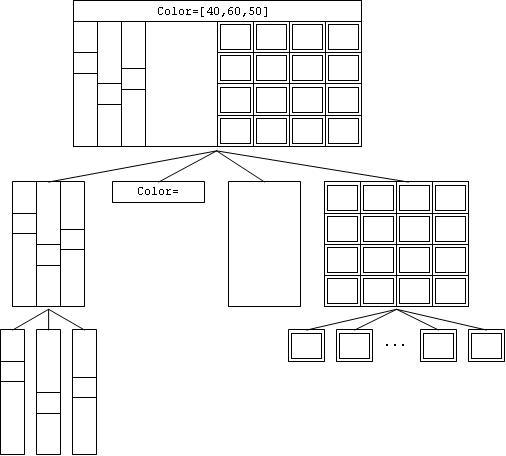
\includegraphics[scale=0.4]{compound-window.png}
\caption{复合窗口}
\label{fig:compound-window}
\end{figure}

和正则表达式一样,窗口也可以作为其他窗口的一部分。例如,如果要定义一个窗口,左边有3个滑块,中间有一个绘图板,16个按钮4个一组地依次排列在右边,文本框排列于顶部。我们通过把简单的窗口放置在较为复杂的窗口中,就能够实现这一需求。




大多数计算机程序本身就可以看成是复合的产品,这时方法或者过程的调用就是复合的机制。

实际上,从语言的基本语句开始(赋值等),通过复合法可以建立一个实用的函数库。以这些函数库为基础,就可以形成更加复杂的函数。如此继续下去,每一层都建立在上一层的基础之上,直到最终完成所要求的应用程序。

抽象通常与组件(component)划分相联系,组件封装了某种主要特征,并通过简单和固定的接口(interface)与其他组件相互作用。

组件的划分意味着我们可以把一项大任务分成一个个的小问题,这样这些小问题就可以大体上相对独立地进行解决,提供符合接口要求的实现(implementation)是每一个组件开发者的责任。

\section{Specialization}



另外一个处理复杂问题的方法是使用特化分层来构建抽象,有时也把它称为分类系统。例如,在生物学上把生物分为动物和植物,动物又分为脊椎动物和无脊椎动物,脊椎动物包括哺乳动物,哺乳动物包括狗、马、鲸鱼等。

\begin{quote}
\texttt{这种分类同时也存在特例,鸭嘴兽是产蛋的哺乳动物,因此如果我们把这种特殊现象与哺乳动物生产幼仔来繁衍后代的特征相联系,就需要更改鸭嘴兽的特征来解释为什么鸭嘴兽属于哺乳动物,却能够产蛋的事实。}
\end{quote}






面向对象语言也需要一种特化分层机制,来改写从更加普遍的类别继承而来的信息,这就需要更加深入地讨论类继承的思想。

使用特化分层抽象与以前的抽象之间的主要区别在于越特化的抽象层次是越普遍化的抽象层次的表现。不过,与前面所使用的从肌肉的特性抽象到各种化学作用的描述时的观点是不同,因此这两种不同的关系可以描述成是(is-a)继承关系和有(has-a)继承关系。

实际上,使用任何一种抽象类型的原因都是一样的。抽象的原则允许我们忽略某些细节,以便更易于表现少数几个主要的特征。



同样的技术也应用在面向对象语言,新的接口从现有的接口上形成。一个类从已有的类那里继承而来,这时和原始类相关的所有特性(数据字段和行为)都同样适用于新类。




在Java AWT(Abstract Windowing Toolkit)库的案例中,当使用AWT创建一个新的应用程序时,主类作为Frame的子类,依次地和AWT库的其他类链接。

\begin{figure}[htbp]
\centering
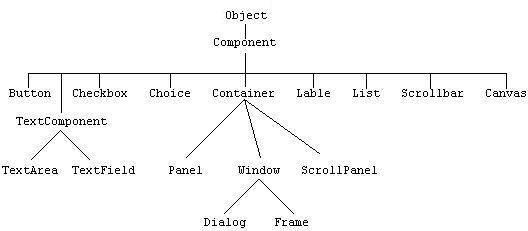
\includegraphics[scale=0.5]{awt-example.png}
\caption{Java AWT类层次}
\label{fig:java-awt-example}
\end{figure}

Frame是应用程序窗口的一种特殊类型,但是它也是Window类的一种更特殊的形式。Window可以包括其他的图形对象,因此它也是一个Container类型。

每一个继承层次都为更低的层次提供方法,即使最简单的应用也需要使用如下的方法。

\begin{table}[htbp]
\centering
\begin{tabular}{ll}
setTitle(string)	&从类Frame继承而来\\
setSize(int,int)	&从类Component继承而来\\
show()			&从类Window继承而来\\
repaint()			&从类Component继承而来\\
paint()			&从类Component继承而来,将在新的应用程序中被改写\\
\end{tabular}
\end{table}



分类系统——在面向对象语言中更倾向于使用继承层次(inheritance hierarchy)这个术语。其中,层次是一个普通类别的更详细的表示,每一层次都是上一层次更加特殊的表现。例如,一个类型系统的例子就是生物学上的分类,其中更一般层次的知识适用于那些更特殊层次的对象。

如果将继承层次技术用于软件系统时,可以大大简化新组件的创建。

\begin{compactitem}
\item 新组件和已有的类别相关;
\item 新组件可以自由地利用已有类别的所有功能(例如Java类库中的Frame组件)。
\end{compactitem}


\chapter{Pattern}

当面对一个新问题时,大多数人会首先看一看他们曾经解决过的问题和现在的新任务有什么共同的特征,因此那些原来的问题可以作为一种模式,新问题也将以相似的方式进行处理,只需针对不同的环境做一些必需的改动,这一观察结果暗示了软件模式(Pattern)的思想。

\begin{quote}
\textsl{模式就是试图为问题提出一个已经被证实的解决方案,以便于能够很容易地用类似的方式来解决以后的问题。在面向对象领域,这一思想广泛地用来描述对象团体中成员之间的相互作用模式。}
\end{quote}

下面用一个简单的例子证明模式的这一思想。假设正在开发一个网络应用程序,这意味着应用程序的一部分运行于一台计算机,另一部分运行于通过网络连接着的另外一台计算机。在这两台计算机之间建立实际的连接和通过连接传递信息这些细节,可能与应用程序的大部分应用都毫不相关。

构建上述这些关系的一种方式就是使用一种称为代理的模式,代理是一种将网络连接隐藏于其中的中介。

对象可以和代理相互作用,但却完全感觉不到代理内部使用哪种具体的网络连接类型。当代理接收到一项关于数据或者行为的请求时,它把这些请求打成一个包,通过网络进行传输,然后接收到响应包,解包,再将响应信息返回给客户。

通过代理模式完成客户请求时,实际上客户完全感觉不到网络协议的细节。
\[\mbox{\fbox{客户}}\longrightarrow \mbox{\fbox{代理}} \longrightarrow \mbox{\fbox{服务器}}\]

需要注意的是,这种模式的描述是如何抓住交互的关键点(对客户隐藏通信协议的需要),而忽略交互的其他方面的(例如在客户和服务器之间传递的特定的信息)。

\begin{quote}
\textsl{模式是对某些已经在多个地方、以多种形式出现过的问题的解决方案的概括性的描述,说明了如何确定问题,同时解释了采用某种解决方案和考虑其他替代方法的原因。}
\end{quote}




\chapter{Language}


面向对象技术并不是革命性地,它只是从模块到抽象数据类型最终到对象这个发展过程地自然结果,因此从汇编语言到面向对象编程语言的本质都是抽象机制。



\section{Assembly}





在使用机器语言进行编程时,存储单元使用地址进行描述,无法按照名称或目的来描述。

类似地,运算使用数字操作码进行描述。例如,整数加法使用操作码33,整数减法使用操作码35。


下面的示例把地址372中的内容加到地址376中的内容上,然后从结果中减去地址377中的内容。

\begin{lstlisting}[language=bash]
33  372  376
35  377  376
...  
\end{lstlisting}


相比机器语言,汇编语言允许使用符号名称,因此可以使用汇编语言对上述示例进行改写。

\begin{lstlisting}[language=bash]
ADDI  A, X
SUBI  B, X
...
\end{lstlisting}


汇编语言本身是对机器语言的抽象,而且汇编语言和过程作为抽象机制把用户的视角集中在功能层次上——如何完成一项任务,从而使编程更加人性且友好。


\section{Procedure}

过程和函数代表编程语言抽象的进一步改进。其中,过程提取重复执行的任务的定义用以复用,而且过程还为信息隐藏提供了可能,这样其他用户就可以通过接口来调用过程,无需了解其实现的确切细节。

下面以堆栈为示例进行说明,首先需要建立工作的可视接口(即init、push、pop和top例程),然后确定合适的实现技术(例如包含栈顶指针的数组、链表等)。



\begin{lstlisting}[language=C]
int datastack[100];
int datatop=0;

void init(){
	datatop=0;
}

void push(int val){
	if(datatop<100){
		datastack[datatop++]=val;
	}
}

int top(){
	if(datatop>0){
		return datastack[datatop-1];
	}
	return 0;
}

int pop(){
	if(datatop>0){
		return datastack[--datatop];
	}
	return 0;
}
\end{lstlisting}

在使用过程来实现上述例程时就会发现,4个例程中的任何一个都不能局部创建堆栈本身所包含的数据,它们必须共享这些数据。如果选择只能是局部变量或者全局变量,那么堆栈数据只能保存在全局变量中。

使用过程式程序设计语言来实现堆栈等数据结构时,如果变量是全局的,就无法限制其可存取性和可视性。例如,如果使用数组datastack来表示堆栈,那么所有用户都可以对其进行修改,而且任何人都可以创建同名变量,从而产生冲突错误。

类似地,上述init、push、pop和top也必须保留为专用,不能被其他部分的程序用于其他目的(即使那些代码和堆栈例程毫无关系)。

实际上,过程并不是所有问题的答案,尤其不是信息隐藏的有效机制,只是部分地解决了多用户使用相同名称的问题。


\section{Module}


为了解决全局名称空间拥挤的问题,从过程和函数中继续抽象产生了模块的思想。

在某种程度上,模块可以简单地看作是用来改善建立和管理名称集合及其相关数值的技术,其中堆栈就是典型的例子。

使用模块来实现堆栈时,可以包含希望广泛公开地被外界获取地信息(接口例程),同时也可以包含对用户进行存取控制的其他数据值(堆栈数据本身)。

简而言之,模块提供了将名称空间划分为公有和私有两个部分的能力,其中:

\begin{compactitem}
\item 公有部分可以从模块外存取;
\item 私有部分只能从模块内存取;
\item 类型、数据(变量)和过程可以在任何部分定义。
\end{compactitem}

下面的示例说明了关于堆栈抽象的模块封装。

\begin{lstlisting}[language=bash]
module StackModule;
	export push, pop,top; (* the public interface *)
	
	var
		(* since data values are not exported, they  *)
		datastack : array [1 .. 100] of integer;
		datatop : integer;
	procedure push(val : integer) ...
	procedure top : integer ...
	procedure pop : integer ...
	begin  (* can perform initialization here *)
		datatop = 0;
	end;
end StackModule.
\end{lstlisting}

David Parnas对模块提出了以下两条基本原则,从而实现了明确且有意识的信息隐藏(information hiding)。

\begin{compactenum}
\item 模块必须为目标用户提供得以正确使用模块所需的所有信息,除此之外,无需提供其他任何信息。
\item 模块必须提供完成模块所需的所有信息的实现,除此之外,无需提供其他任何实现。
\end{compactenum}

模块解决了一些问题,但是并没有解决全部问题。例如,模块本身提供了一种有效的信息隐藏的方式,但是模块不允许用户实现实例化(instantiation)。

实例化是一种能够建立数据区域多份拷贝的能力,因此需要引入更高级的抽象机制来解决实例化问题。

\section{ADT}

抽象数据类型(Abstract Data Type)使得用户可以定义和使用自己的新的数据抽象,而且还可以为用户提供能够创建多个数据类型实例的能力。

抽象数据类型和系统基本数据类型的工作方式相同,并且用户只需要知道实例所提供的操作就可以直接使用,无需关心这些操作是如何实现的。

ADT通过抽象规范进行定义,例如堆栈数据类型的规范包括入栈(push)、出栈(pop)和返回栈顶(top)等操作,而且与ADT匹配的是一个或多个不同的实现方式。

使用ADT来定义堆栈时,可以有多种不同的实现技术(例如数组或链表),但是它们对外的操作都是一致的。

ADT的进化在于隔离了接口的概念和实现的概念,而且模块仍然可以作为ADT的实现技术来使用。

虽然ADT和模块具有相关性,但是不再完全相同,因此要建立一个抽象数据类型时必须要做到以下几点:

\begin{compactenum}
\item 导出一个类型定义;
\item 生成一套可用的操作,可以用来操纵类型的实例;
\item 保护与类型相关的数据,使得只有通过所提供的例程才能操作这些数据;
\item 建立类型的多个实例。
\end{compactenum}

在定义抽象数据类型后,模块仅仅用于信息隐藏机制,这样用户就可以直接定位到上述第2条和第3条内容,第4条要求可以使用合适的技术来实现。例如,在CLU语言和Ada语言中使用的包(Packages)就可以更加直接地定位到具体地抽象数据类型。



\section{Service}



随着程序开发逐渐向模块和ADT的延伸,计算从以功能为中心转变为以数据为中心,从而使数据的重要性表现为它们的结构、表示和操纵。

面向对象编程从以数据为中心的角度来看待世界的观点开始,继续向前发展为以服务(service)为中心,并提供给程序的其他部分。

\begin{compactitem}
\item 汇编语言
\item 函数和过程(以功能为中心的观点)
\item 模块
\item 抽象数据类型(以数据为中心的观点)
\item 面向对象编程(以服务为中心的观点)
\end{compactitem}

在某种程度上,一个对象就是一个简单的抽象数据类型,或者说一个对象定义就是一个抽象数据类型。

\begin{quote}
\texttt{面向对象编程的概念是建立在抽象数据类型思想上的,并且增加了代码共享和代码可复用性这一重要的创新。}
\end{quote}

其他类型的抽象也可以用类似的方法进行定义,不再根据它们特定的行为或者数据值,而是根据它们所提供的服务。

关于如何构建一个计算机程序的观点从以功能为中心开始,发展到以数据为中心,最后以服务为中心,因此面向对象编程代表了上述发展过程的第3步。

除了计算以服务为中心的观点外,面向对象编程还在抽象数据类型的概念上增加了几个重要的新的思想。其中最重要的就是消息传递(message passing)。

活动是通过对特定对象的请求(request)初始化的,而不是通过对特定功能的调用初始化的。


隐藏在消息传递中的思想是消息的解释(interpretation)可以随着对象的不同而改变,即消息所导致的行为和响应依赖于接收信息的对象。



面向对象编程还增加了继承(inheritance)机制和多态(polymorphism)机制。

\begin{compactitem}
\item 继承允许不同的数据类型共享同一代码,从而可以减少代码量,并且增加代码的功能。
\item 多态允许这些共享代码被定制成适合某一数据类型的特定环境。
\end{compactitem}

例如,push对于堆栈是一个含义,对于机械式手臂控制器却是另一个完全不同的含义,因此操作的名称不需要惟一,使用简单而直接的命名形式有助于创建更容易阅读和理解的代码。

对于组件独立性的强调有助于软件的增量开发,在这一过程中,每个软件单元在合并成一个大系统之前,都可以独立地进行设计、编码和测试。

面向对象设计不同于传统的软件设计,它的驱动力是对不同软件组件分配责任。如果没有主体去执行动作,就不会有行为发生,因此每一个行为都必须指定给对象集合的某个成员。反之,对象集合中成员完成的行为要能够实现所期待的目标。


服务提供者(service provider)的概念在开发复杂软件系统时是非常有用的,软件组件为和它相互作用的其他组件提供服务。

在现实生活中,我们经常通过成员提供的服务来刻画团队成员的特征(例如速递员负责把花从花商那里送到顾客手上),因此这一比喻可以让我们用日常生活中思考问题的方式来考虑一个大规模软件系统。


\chapter{Design}

使用面向对象语言(即支持继承、消息传递和类的语言)既不是进行面向对象编程的充分条件,也不是必要条件。

OOP最重要的方面是如果构建一个由大量的在很大程度上自治的且互相作用的个体所组成的体系,因此为了构建这样一种体系,就需要借助于目标驱动设计方法和责任代理驱动设计方法等。

责任代理驱动设计方法由Rebecca Wirfs-Brock提出,它是最简单的、便于从设计到编程过渡的面向对象设计技术之一,另外还有由统一建模语言(UML)表示的符号技术。

\section{Responsibility}

责任是一把双刃剑。当你确定一个对象(比如是一个软件系统)要对某些特定行为负责时,往往希望它必然能够表现出符合相应规则的行为来。


更重要的是,责任意味着一定程度上的独立或者无干扰。如果你告诉一个孩子,他有责任打扫他自己的房间,这就意味着在他开始打扫房间之前你不必对他进行督促,否则有悖责任的本质。

我们希望的是,只要以一种正确的方式将指令传递给对象,就会产生预期的结果,而且对象自身也希望能够自由地执行责任而不受干扰。

同样,当Chris要求花商把花送给Robin 时,他也没有必要停下自己的事情来考虑花商如何去送花。花商对这项任务负有责任,他可以自由地履行责任而不受来自顾客Chris的干扰。

传统的编程与面向对象编程之间的差异,在某种程度上,就像一个孩子在做一件事情时对他积极地督促和委派他去对某件事情负责的区别一样。

对于传统编程,大多是这样的情况:一件事情的发生依赖于另外一些事情的发生——比如修改一个记录或者更新一个数组等,因此软件系统中的一部分代码通常是通过控制器或数据连接与系统的其他部分进行密切联系的。

从本质上来说,传统编程中的依赖关系需要通过使用全局变量、使用指针值或者是依靠代码其他部分的实现细节等各种不恰当的方式来实现。

责任驱动的设计应该完全去除这些连接,或者至少尽可能地使它们不那么显著,而且责任驱动设计在传统语言编程中也是十分重要的。

责任驱动设计将信息隐藏从技术提升到艺术,当从小项目过渡到大项目时,信息隐藏的原则将至关重要。


面向对象编程的主要优点之一是在进行下一个项目开发时复用软件子系统。例如,一个模拟管理程序既可以对台球桌上的台球进行模拟处理,也可以对鱼缸中的鱼进行模拟处理。

使用面向对象编程技术产生的代码复用的能力意味着软件几乎不需要熟悉特殊领域相关的组件,就完全可以将与特殊领域行为相关的责任委托给系统的指定应用程序去处理。

独立项目的开发与可扩展软件系统的开发之间的差异通常被描述成小项目编程和与之相对的大项目编程之间的差异。其中,小项目编程具有以下特性:

\begin{compactenum}
\item 代码由一个程序员或者由一个很小的团体来编写。
\item 每个开发成员都理解项目的所有细节(从上到下,从开始到结束)。
\item 软件开发过程中的主要问题是设计和开发解决当前问题的算法。
\end{compactenum}

另一方面,大项目编程具有以下特性:

\begin{compactenum}
\item 软件系统由一个大型团队开发,团队通常由具有不同技能的人员组成。
\item 不同的人员负责不同的任务,分别包括系统的规范或设计、独立组件的编码,以及不同组件的集成以形成最终产品。
\item 没有哪个人能够对整个项目完全负责或者能够理解整个项目的方方面面。
\item 软件开发过程中的主要问题是细节的管理和保障项目的不同分工人员之间信息的有效交流。
\end{compactenum}

软件设计过程都是从行为分析开始的,因为人们往往最先了解系统行为而不是其他的方面。

早期的软件开发方法学主要集中关注的是如何设计基本数据结构和如何规划函数调用的总体结构,这些内容通常都包含在关于应用程序的正式规范中。但是,只有在对相当数量的问题分析之后,才能确定应用程序的结构化元素。

同样,一份正式的规范通常以一份既不会被程序员也不会被客户所理解的文档来体现。但是,行为却在设想的开始就能被描述出来,并且(不同于正式的规范)能够用程序员和客户都能理解的术语来描述。

由Rebecca Wirfs-Brock发明并首次描述的责任驱动设计技术(Responsibility-Driven Design,RDD)是一种面向对象设计技术,该技术由各个级别行为的重要性所驱动,现在仍然是一种不可替换的设计技术。


在一个软件设计师眼中,在开发交互式智能厨房助手的RDD实例中,首先确定的是交互式智能厨房助手的示意图。

\begin{figure}[htbp]
\centering
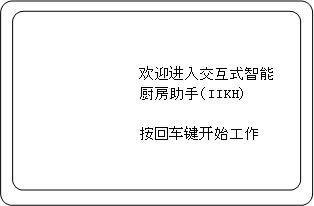
\includegraphics[scale=0.65]{rdd-example.png}
\caption{IIKH}
\label{fig:iikh}
\end{figure}


简单地讲,交互式智能厨房助手(the Interactive Intelligent Kitchen Helper,IIKH)是一个基于PC的应用程序,它将取代在通常厨房中所使用的食谱索引卡系统。除了维护食谱数据库之外,IIKH还可以帮助确定一段时间内的饮食计划——比如一个星期内的计划。IIKH的使用者可以通过软件的终端浏览食谱数据库,以交互的方式创建一系列新菜谱。IIKH会自动针对原料的种类和数量来调整食谱。为某一周、某一天或者是某一餐打印出菜谱清单,而且还能打印出一段时间内的食谱所需要的所有原料的详细清单。


事实上,大多数软件系统的最初描述和IIKH一样,在初始阶段,系统规范在很多关键点上的描述都非常模糊。

另外一个事实是,无论如何,软件系统的最终设计和开发要靠多人的协同合作,因此设计小组的初始目标是必须澄清描述中的模糊之处,将项目合理地划分成多个组件并分配给每个小组成员进行开发。

面向对象编程的基石是将软件通过行为(action,即将要执行的动作)使之特性化,将在每个系统的各个级别的开发上都得以体现。

最初,小组会通过很高级别的抽象手法来特性化整个应用程序的行为。由此产生了不同的软件子系统的行为描述。只有当所有的行为都被确定和描述之后,软件设计小组才能进入编码(coding)阶段。

强调行为是面向对象编程的一个标志,在系统的最初描述中就可以确定行为,远远早于能够确定其他设计观点的时刻。

由于不断地被行为所驱动,因此从问题描述开始,通过软件架构、代码开发直到应用程序完成,责任驱动设计可以实现这个过程的平稳过渡。

\section{Scene}


第一个任务就是细化软件规范。最初的规范,除了一些最宏观的概念外,总是存在大量的模棱两可和不确切的方面。这一步就几个目标,其中一个目标就是能够对最终产品的表象(外观和感觉)进行更好的控制。

这些信息可以反馈给我们的客户,然后看看他是否同意我们的构思。最终应用程序的规范在软件系统的构建过程不可避免地要经常更改,因此重要的是软件的设计要能够适应变化,并且尽早地注意潜在的变化。

同样重要的是,现在所做出的非常高级别的决策抽象会影响到最终软件系统的结构,而且特别要注意的是,我们在设计中将要执行的活动会体现出各个组件的内部结构。

为了揭示系统的基本行为,我们的设计小组首先建立了一系列场景,即将应用程序的运行情况通过场景来模拟表示,就像已经拥有了一个正常工作的系统一样。



一个复杂的物理系统工程,可以通过将其分解成更小的单元而简化设计。同样,软件工程也可以通过标识和开发软件组件来简化软件系统设计。

组件仅仅是抽象的实体,它可以执行一定的任务(即完成一定的责任)。从这方面来讲,没有必要精确地了解组件的详细描述,也没有必要了解组件执行任务的细节。

一个组件最终可以转变成一个函数、一个结构、一个类或者是其他组件的集合。在这个开发层次上,组件有以下两个重要的特性:

\begin{compactitem}
\item 组件必须拥有一套小的且定义明确的责任集合;
\item 组件应该尽可能地减少与其他组件的交互;
\end{compactitem}


当设计小组遍历完他们所设计的所有场景之后,便开始对将要执行某项任务的组件进行标识。每一项必然发生的活动都要被标识,并且作为责任分配给某一组件,如下图所示。


\begin{table}[htbp]
\centering
\begin{tabular}{|l|l|}
\hline
组件名称 & 协作组件\\
\hline
分配给该组件的责任描述&其他组件列表\\
\hline
\end{tabular}
\end{table}

在软件需求分析过程中,可以用小型索引卡来表示组件,索引卡上写明软件组件的名称、组件的责任以及必须与该组件交互的其他组件。

CRC卡是由Beck发明的,CRC代表了Component、Responsibility和Collaborator,即组件、责任和协作组件,CRC卡与每一个相应的软件组件关联,上面记录了该组件的责任。

通过场景工作时,有必要将CRC卡分配给设计小组的不同成员,持有代表组件的CRC卡片的成员需要记录与卡片相关联的软件组件的责任,并且在场景模拟期间担任软件“代理人”的角色。当软件系统需要另外一个组件的服务时,他(或她)描述软件系统的活动,将“控制”传送给其他成员。

使用CRC卡可以对各种不同的软件设计方案进行试验、研究或弃用。

卡片的物理分离可以加深设计人员对不同组件之间的逻辑分离的重要性的理解,而组件之间的逻辑分离可以强化内聚性和耦合性,同时CRC卡的版面限制也是估量软件系统的复杂程度的量度。

如果一个组件的CRC卡所提供的版面无法容纳这个组件需要执行的任务,那么这个组件可能是过于复杂了,这个时候设计小组应该寻找更加简单的解决方案,实际应用中可以通过将部分责任转移到其他组件,从而将一项任务分配给两个或者更多的新组件。


在小组讨论时,组件的标识发生在对工作系统的执行情况进行构想的过程中,这个过程的进行通常是通过循环来回答“什么/谁”这个问题。

首先,设计小组确定下一步执行什么活动,紧接着就要回答谁来执行这项活动这个问题。以这种方式设计一个软件系统,与组织一群人(例如俱乐部)很相似。


任何将要执行的活动都必须以责任的形式赋予给某个组件。只有分配一个主体去执行一项行为,这项行为才能发生。这也如同一个俱乐部的运行,任何活动的执行都必须分配给某些个人,在组织一个面向对象系统编程的过程中,所有的活动都必须分配给某些组件来负责。优秀的面向对象设计的秘诀就是先对每项活动建立一个主体。

\section{Document}

从场景分析阶段开始,就应该认识到,有两份文档应该是任何软件系统的基本组成部分:用户手册和系统设计文档,这两项工作需要在编码之前开始。

用户手册从用户的角度描述了用户与系统之间的相互作用,这是一种验证开发小组对应用程序的理解与用户对应用程序的理解是否一致的有效手段。在创建场景中所作的决定应该密切符合用户对最终应用程序要求,因此用户手册的开发要紧跟场景开发的进程。

在任何实际代码开始编写之前,软件设计小组对应用程序的理解与最终用户十分接近。这样软件开发者才能够很容易地理解那些对于初学者用户需要解决的问题。

用户手册同时也是一个优秀的工具,它可以验证开发小组看待问题的方式与客户是否相同。客户很少能够给开发小组提供一份详细而正式的规范,因此,客户和开发小组之间需要进一步确认的问题和相互的交流应该在正式编程开始之前就尽早进行,这样可以防止以后出现大的分歧。

第二个基本文档是设计文档,设计文档记录了软件设计中的主要决定,这些决定应该在设计者对各项要求都思路清晰的情况下产生,而不是在许多相关细节都快忘记之后才进行设计。在开发阶段早期,通常很容易书写软件系统的全局描述。但是很快,开发工作的重心会转移到每个组件或者模块的级别上。尽管进行模块级文档设计也是很重要的事情,但是,如果设计文档过多地关心每个模块的细节,将使以后的软件维护人员很难对软件系统的整体结构形成一个概要的了解。

CRC卡是设计文档的一个方面,但是许多其他重要的决定并没有通过它反映出来。任何关于主要设计的支持或反对的讨论,以及影响最终决定的因素都应该记录下来。应该维护项目进度的日志和日记,而且在整个开发过程中,用户手册和设计文档也要随着软件的不断改进而即时地改进,保持与软件同步。

\section{Action}


在场景设计阶段,开发小组决定在系统开始时,呈现在用户面前的是一个吸引人的信息丰富的窗口。我们将展示这个窗口的责任分配给一个叫做Greeter(问候者)的组件来完成。

通过某种还未确定的方式(可能是下来菜单、按钮、按键或者显示屏),用户可以从几项活动中选择一项。最初,开发小组只确定了五项活动:

\begin{compactitem}
\item 自由浏览现存食谱的数据库,但是不涉及任何特定的就餐计划;
\item 对数据库增加新食谱;
\item 编辑或注解一个已有食谱;
\item 检查已存在的食谱计划;
\item 建立一个新的食谱计划;
\end{compactitem}

这些活动可以分成两组:前三条与食谱数据库有关,后两条与饮食计划有关,因此开发小组下一步决定创建与这两项责任对应的组件。

继续场景,开发小组选择暂时忽略就餐计划管理,先着手细化Recipe Database(食谱数据库)组件的活动。例如,下面显示了用来表示“问候者”组件的最初的CRC卡。

\begin{table}[htbp]
\centering
\begin{tabular}{|l|l|}
\hline
问候者			&协作组件\\
\hline
显示丰富的初始化信息&	数据库管理者\\
\hline
为用户提供活动选择&	计划管理者\\
\hline
食谱数据库管理者 & \\
\hline
计划管理者 & \\
\hline
\end{tabular}
\end{table}



泛泛地讲,食谱数据库组件的责任就是维护食谱集合。现在,已经可以确定这项任务的三个要素:食谱数据库组件必须便于浏览现有的食谱库、编辑食谱以及增加新食谱到数据库。


有很多关于如何让用户更好地浏览数据库的问题必须到最后才能决定。比如,最初是否应该展现给用户食谱分类清单(如汤、沙拉、主食和甜点等)?用户在输入关键字进行限定搜索时,是通过提供配料清单选择当前关键词,查看所有包括这些配料(例如杏仁、草莓和奶酪)的食谱,还是通过提供以前的搜索关键词(例如Bob最喜欢的蛋糕名称)来选择当前关键词进行搜索?

思考上面这些问题会很有意思,但是最重要的地方却是不需要在此时对这些问题做出决定。因为它们只影响一个单独的组件而不影响系统其他功能,继续场景时应该忽略这些,假定用户通过某种方式已经选中一个特定的食谱。


永恒不变的就是偶然与变化的必然性,在软件开发中也是如此。无论我们怎样认真仔细地进行软件系统的设计,几乎可以确定的是,在系统开发的某一时刻,用户的需求会发生改变,并强求软件做出相应的变化。软件开发人员和软件设计人员都需要预测这些变化,并且做出相应的变化。


\begin{compactitem}
\item 基本原则是变化影响尽可能少的组件,即使是应用程序的外观或者功能发生大的改变,也应尽量只改变代码的一至两个部分。
\item 尽量预测可能发生变化的源头,并通过尽可能少的软件组件将这种变化的影响隔离开来。最可能发生变化的来源有界面、通信方式和输出格式等。
\item 尽量隔离或减少软件对硬件的依赖。例如,应用程序中的食谱浏览界面可能部分依赖于系统运行的硬件平台,但是未来软件发布时可能需要移植到不同的平台。一个良好的设计应该预测到这些变化。
减少软件组件之间的耦合性会降低组件之间的依赖性,当其中一个组件发生变化时,与之相关的组件能够尽可能地减少影响。
\item 设计文档应该详细记录所有主要决定的设计过程和讨论记录。与发布最初软件版本时相比较,在发布未来软件版本时,几乎可以肯定地是,软件维护人员或设计人员将发生部分变动。设计文档应该使未来的每一个小组成员都了解每一项决定背后的重要因素,帮助他们避免花费时间来讨论一些已经解决过的细节。
\end{compactitem}

每一个食谱都与一个特定的食谱组件相关联,一旦选定一个食谱,控制信息就会传送到相关的食谱对象。

一个食谱必须包含确定的信息,基本上包括配料清单和将配料做成最后食品的操作步骤。在我们的场景中,食谱组件还需执行其他活动。例如,它将以交互的方式在屏幕上显示食谱,并且用户可以被授权注解或改变配料清单和操作步骤,用户还可以选择是否打印食谱。所有这些行为都是Recipe(食谱)组件的责任。

现在,我们将继续讨论独立形式的“食谱”组件。在设计的过程中,可以把它看作是代表许多实际食谱的原型食谱,以后我们将继续进行独立组件和多重组件的对比讨论。

通过上面的分析可以知道,允许用户浏览数据库是一项必然发生的行为。

现在,我们将开始分析数据库管理组件,假定用户希望新增一个新的食谱,数据库管理组件以某种方式将新食谱加入某一类别中,要求用户录入新食谱的名称,然后创建一个新食谱组件,显示供用户编辑的空白输入框。因此,执行这项新任务的责任是允许用户编辑已有食谱的责任集合中的一个子集。

分析完浏览和创建新食谱后,下面将分析“问候者”组件,研究每日食谱计划的开发,这是Plan Manager(计划管理者)组件的任务。

用户能够以某种方式保存已有计划,因此用户即可以从检索一个已创建的计划开始,也可以从创建一个新计划开始。在后一种情况下,用户将面对一些计划的日期,每一个日期都与一个独立的Date(日期)组件相关。

用户可以选择一个特定的日期来进一步查看,这时控制就会传送到相应的“日期”组件。“计划管理者”的另外一项活动就是打印出计划期间的食谱。最后,用户可以指示“计划管理者”组件列出这些食谱所需的全部杂货。

“日期”组件需要维护每一餐的集合以及用户提供的备注信息(生日聚会、周年庆典、纪念宴会等)。日期组件还要打印关于指定日期的信息。通过某种方式,用户可以要求“日期”将关于指定日期的所有信息打印出来,或者选择进一步查看就餐细节。在后一种情况下,控制将传送给Meal(膳食)组件。

\begin{compactitem}
\item “膳食”组件维护扩展食谱集合,这里“扩展”是指用户增加一倍、两倍或者一个食谱。
\item “膳食”组件显示关于一餐所用的全部食物信息。用户可以从中添加、删除任何食谱,也可以将信息打印出来。
\end{compactitem}

为了发现新的食谱,必须让用户能够浏览食谱数据库。因此,“膳食”组件就必须与食谱数据库组件交互。设计小组以这种形式继续研究各种可能的场景。

到现在为止,我们还没有设计开发的场景主要就是关于如何处理例外情况。例如,一个用户选择搜集一个食谱的关键词,却没有与之相匹配的食谱,这时系统就需要确定该如何将这种信息反馈给用户。还有就是如果一个用户取消某个搜索行为,例如,用户输入一个食谱名称开始搜索之后,却又放弃了该搜索。每一种情形都应该考虑进去,处理不同情况的责任要分配给一个或更多的组件去执行。

设计完成各种场景之后,软件设计小组最后决定将所有的活动适当地分配给6个组件来完成,其中:

\begin{compactitem}
\item “问候者”组件只需与“计划管理者”组件和“食谱数据库”组件进行通信。
\item “计划管理者”组件只需与“日期”组件通信,“日期”组件只需与“膳食”组件进行通信。
\item “膳食”组件与“食谱管理者”组件进行通信,并且通过这个代理,与特定的食谱进行通信。
\end{compactitem}

\begin{figure}[htbp]
\centering
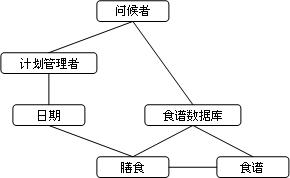
\includegraphics[scale=0.65]{rdd-example-component.png}
%\caption{}
%\label{rdd-example-component}
\end{figure}

对于难以定义的问题,基于行为的设计技术要比基于数据结构的设计技术更易于使用。

\section{Diagram}

在表明组件之间的静态关系后,不过仍然不适合描述在场景执行过程中组件之间的动态关系,描述组件之间动态关系的更好的工具就是交互图表。下图显示了交互式智能厨房助手的交互图表的开始情况。



\begin{figure}[htbp]
\centering
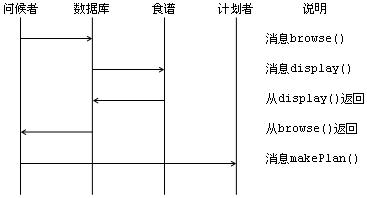
\includegraphics[scale=0.65]{rdd-example-diagram.png}
%\caption{}
%\label{rdd-example-diagram}
\end{figure}


在图表中,从上到下表示时间从后到前。每个组件由一条垂直线来表示。用从一条垂直线指向另一条垂直线的水平箭头线来表示一个组件将一条消息传递到另外一个组件。类似地,组件返回的控制或返回调用者的结果值也用箭头线来表示(有时候也用两种不同的箭头形式来表示,比如用实线表示消息传递,虚线表示返回控制)。图表右侧的说明更加详细地解释了正在进行的交互。

通过时间轴,交互图表可以更加清晰地描述场景中事件的顺序。因此,交互图表是用于复杂软件系统的有效文档工具。


\section{Component}


\section{Action \& State}



组件通过行为,即通过它能够做什么来表现它的特征,但是同时组件也可以包含确定的信息。把IIKH中的一个“食谱”结构作为原型组件,查看这样的组件的一种方式就是把它看作是一个由行为和状态组成的对象。


\begin{compactitem}
\item 组件的行为是指组件所能执行的一系列动作。对一个组件所有行为的完整描述有时称为协议。对于“食谱”组件来说,协议所包含的行为有编辑准备命令、在终端屏幕上显示食谱或打印食谱等。

\item 组件的状态是指某一特定时刻组件所包含的所有信息。对于“食谱”组件来说,状态包括配料和准备指令。
\end{compactitem}

状态不是恒定的,而是可以随时间变化的。例如,用户通过编辑一个食谱(行为),可以改变准备指令(部分的状态)。

不是所有的组件都必须维护状态信息。例如,可能有这样的情况,由于“问候者”组件不需要在执行过程中记录任何信息,因此它可以没有任何状态信息。然而,大部分组件都是由行为和状态结合而成的。

\section{Instance \& Class}


状态和行为的分离使我们澄清了在以前的讨论中所避开的观点。需要注意的是,在实际的应用程序中可能会有很多不同的食谱。然而,所有这些食谱都会以同样的方式执行其行为,也就是说,每个食谱的行为都是相同的,只有状态——各种配料清单和准备命令——对于不同的食谱是不一样的。在开发的早期,我们的注意力应集中在所有食谱的共同行为特征上,每一个食谱的特定细节并不重要。

\begin{quote}
\textsl{类用来描述一系列有相似行为的对象。}
\end{quote}

在几乎所有的面向对象语言中,类还用于语法结构,类的具体表现个体称为实例。

行为是和类相联系,而不是和个体相联系。也就是说,一个类的所有实例都以相似的行为来响应同一命令。

另一方面,状态是个体的特性,我们可以在“食谱”类的各个实例中看到这一点,它们都能执行相同的动作(编辑、显示、打印),但是,使用的数据却是不同的。

\section{Coupling \& Cohesion}



软件组件设计中的两个重要概念就是耦合性和内聚性。

\begin{compactitem}
\item 内聚性就是一个独立组件的所有责任组成一个有意义的单元的聚合程度。
\item 耦合性描述了软件组件之间的关系。
\end{compactitem}

通过某种方式将一个独立组件的任务联系起来可以使一个组件获得较高的内聚性。可能最常用的联系任务的方式就是通过观察,将存取公共数据值的一组任务放在一起。例如,“食谱”组件的各种责任就是这项原则的一个应用。


一般情况下,由于软件组件之间的联系阻碍了软件的开发、修改或复用的简易性,因此应尽可能地减少耦合的数量。

特别是,当一个软件组件必须访问的数据值(状态)由另外一个软件组件控制时,耦合数量就会增加,应该尽量避免出现这种情况,这将有利于把任务转移到包含必需数据的组件的责任列表中。例如,由于当“食谱数据库”组件执行相关行为时,需要首先编辑食谱,因此设计人员可能会自然地把编辑食谱的责任先指定给“食谱数据库”组件。但是,如果我们这么做,“食谱数据库”代理就需要有直接操作每一个食谱状态(表示配料清单和准备指令的内部数据值)的能力,把编辑食谱的责任转移给“食谱”组件是避免这种紧密联系的一种更好的设计。

\section{Interface \& Implement}


通过行为将一个软件组件特征化,有一个非常重要的结果。一个程序员可能知道如何使用由另外一个程序员开发的组件,但却不需要知道组件是如何实现的。例如,假定把IIKH中的六个组件分配给不同的程序员来开发,开发“膳食”组件的程序员应该允许IIKH用户浏览食谱数据库,并且对某一餐选定一份食谱。要达到这个目标,“膳食”组件只需调用与“食谱数据库”组件相关的“浏览”行为即可,“浏览”行为被定义成返回某一个食谱。这个过程不需要了解“食谱数据库”组件使用的具体实现方式,就可以执行实际的浏览行为。


这种有目的地忽略一个简单接口后面的实现细节的行为称为信息隐藏。我们说,组件封装了行为,它只显示如何使用组件而不显示它执行的细节行为。这自然而然地导致了关于软件系统的两种不同的视角。接口的视角就是指能够被其他程序员看到的界面,它描述了一个软件组件能够执行什么。实现的视角就是指能够被开发特定组件的程序员看到的界面,它描述了一个组件如何完成一项具体任务。


接口与实现的分离可能是软件工程中最重要的概念,然而这对于大多数新手来说仍然是很难理解的。信息隐藏只有在多人合作编程的项目背景下才非常有意义。对于这种工作,限制因素通常不是项目包含代码量的多少,而是程序员之间以及他们各自的软件系统之间的相互交流是否充分。软件组件通常是由各个相互独立的程序员并行地进行开发的。

对于项目开发来说,通用软件组件的复用性变得越来越重要。如果组件成功地复用到系统中,则系统不同部分之间的连接将会减少且容易理解。David Parnas用以下两条原则(称为Parnas原则)来描述这些观点:

\begin{compactitem}
\item 软件组件的开发者必须向目标用户提供所有能用来有效使用组件所提供的服务的信息,而无需提供其他任何信息。
\item 必须向软件组件的开发者提供所有需要用来执行分配给组件的责任的信息,而无需提供其他信息。
\end{compactitem}

接口从实现中分离的结果是,程序员可以在不影响其他软件组件的条件下,对多个具有同一结构、不同实现的组件进行试验。


\section{Formal Interface}

在继续细化组件的开发的过程中,接下来的第一步就是对通信模式和通道进行形式化。应该制订适合于实现每个组件的关于总体结构的设计原则。对于只有一种行为且没有内部状态的组件,可以把它做成一个函数——例如,一个组件只是处理一个字符串,把所有大写字母改成小写字母。

对于执行多项任务的组件,可能更容易用类来实现。对每个组件CRC卡上所标识的责任进行命名,这些名称最终会映射成方法名。与方法名一起,所有传给函数的参数类型也要标识。下一步,还应该描述组件本身的信息,并且对所有的信息都要进行解释说明。如果一个组件需要某些数据项执行一项特定的任务,数据来源(可以通过参数、全局变量值,也可以通过由组件内部维护的局部变量值)一定要明确地标识。

应该仔细思考如何对不同的行为进行命名。Shakespeare曾经说过,一个名称的变化不会改变所描述的对象,但是对于聆听者来说,不是所有的名称都能在头脑中产生相同的想象。

\begin{compactitem}
\item 名称创造了词汇,通过词汇形成最终的设计,因此选择一个有意义的名称是非常重要的。
\item 名称应内部一致、有意义、尽量简短,还要能够让人联想到问题的背景。
\end{compactitem}

通常要花大量的时间去寻找恰当的术语来描述将要执行的任务和操作的对象,而且在设计前期,恰如其分地命名绝对不是一件毫无意义的事情,它可以极大地简化和促进以后的工作。

建议命名时遵循以下基本原则:

\begin{compactitem}
\item 使用可发音的名称,根据经验,如果名称不能被大声地读出来的话,它就不是一个好名字。
\item 用大写字母(或下划线)标出名称中新词的开始,例如命名成“CardReader”或“Card\_reader”,而不是难以辨认的“cardreader”。
\item 仔细检查缩略语,一个对某人来说非常清楚的缩略语,对另外一个人可能比较费解。例如,“TermProcess”是指一个结束的进程还是一个与终端相关的进程呢?
\item 避免有多种解释的名称。“empty”函数是说明一个对象为空,还是清空一个对象的值?
\item 名称中避免使用数字。数字在某些情况下很容易被读成字母(例如“0”与“o”,“1”与“l”,“2”与“z”,“5”与“s”等)。
\item 函数和变量的名称表示布尔值时,可以清楚地表达“真”值或者“假”值,例如“PrinterIsReady”清楚地表明“真”值代表打印机正常工作,但是如果使用“PrinterStatus”无法做到精确。
\item 对于那些代价大且很少发生的操作的命名,要格外注意。这样才可以避免由于错误的函数而引起的错误。
\end{compactitem}


一旦为每一个行为选好名称,就要重新改写每一个组件的CRC卡,写上代表每个确定行为的函数的名称和形参。下图是一个关于“日期”组件CRC卡的例子,只是现在仍未确定的是,每个组件如何执行相关的任务。


\begin{table}[htbp]
\centering
\begin{tabular}{|l|l|}
\hline
日期							&协作组件\\
\hline
							&计划管理者\\
\hline
维护制定日期的信息			&膳食\\
\hline
Date(year,month,day)	——建立一个新日期&\\
\hline
DisplayAndEdit()		——在窗口显示用户可以编辑的日期信息&\\
\hline
BuildGroceryList(List\&)	——把所有膳食的原料增加到杂货列表&\\
\hline
\end{tabular}
\end{table}



确定场景或者角色的模拟应该在更详细的层次上进行,以保证所有活动得以分配,也保证所有必需的信息得以维护且能够被责任组件利用。

在设计表现时,不同于以往,设计团队可以分为几个小组,每一小组负责一个或多个软件组件,任务是将组件描述转化成软件系统的实施。这一过程的主要工作是设计数据结构,每个子系统通过这些数据结构来维护状态信息,进而完成所分配的责任。

数据结构的选择是软件设计过程的核心。一旦选定了数据结构,在完成责任时,组件所使用的代码通常就可以清晰了。但是数据结构一定要与当前的任务相匹配。错误的选择将导致程序复杂而低效,而正确的选择却能达到完全相反的效果。

还应注意,行为的描述也必须转换成算法。这些描述应与协作组件即将执行的任务相匹配,以保证这些任务得以实现,并提供执行每个过程时所需的必要数据。


完成每个软件子系统的设计后,下一步就是实现组件的期望行为。如果前面的步骤执行正确,每一项责任或行为就可以用简要的描述来表示。这一步的任务就是用计算机语言实现所期望的活动。如果没有被早些确定(指作为系统规范的一部分),那么现在可以做出决定的问题都处在一个单独组件的内部。

随着多人协作编程项目变得越来越普遍,由一个程序员来完成一个系统的所有方面的现象变得越来越少。通常,程序员需要掌握的技能就是知道代码的某一部分如何融入整体框架,以及和团队的其他成员如何协同工作。

一般情况下,在组件的实现过程中,将哪些特定信息和行为分配给哪些“隐藏在幕后”的其他组件是很清楚的,从用户的角度来说,软件抽象极少或者没有,因此有时会称这样的组件为facilitators。

将软件子系统逐个实现和测试完成之后,就可以对它们进行集成,形成最终的产品。

组件集成并不是孤立的一个步骤,而是一个过程的某一部分。从一个简单的基础系统开始,逐渐地将各个子系统增加到这个系统中并且使用存根(stub)——没有行为或只有有限行为的简单虚构的例程——对这个还没有生效的部分做测试。

例如,在IIKH的开发过程中,从“问候者”组件开始集成是非常合理的。为了单独测试“问候者”组件,就要为“食谱数据库管理者”组件和日常的“膳食计划管理者”组件编写存根。这些存根的工作仅仅是显示必要的消息和返回。通过这些存根,组件开发小组可以测试“问候者”系统的各个方面(例如,对按键做出正确的响应)。测试独立的组件通常称为单元测试。

紧接着,可以用更加完整的代码来替代一个或更多的存根。例如,开发小组可能决定用实际的系统来代替关于“食谱数据库”组件的存根,同时保持其他部分的存根不动。然后,进一步的测试继续进行,直到系统完全按照所期望的情况来工作(这通常称为集成测试)。
	

当所有的存根都被工作组件代替后,应用软件才最终完成。有意识地减少组件之间联系的设计目标,极大地方便了独立组件的测试,因为这降低了对大规模存根的需要。

在集成过程中经常会出现这样的情况,在某一软件系统中出现的一个错误,却是由另外一个系统中的代码错误所导致的。因此,集成测试将会发现错误,而这又导致某些组件的更改。变更组件后,在进行软件的再次集成(进而,是系统的再次集成)以前,组件应该重新独立测试。当一个组件变更后,这时就需要重新运行以前的测试用例,称为回归测试。


认为应用程序的工作版本一旦交付,软件开发小组的任务就已完成的想法的确很吸引人。但是不幸地是,这几乎从未实现过。软件维护是指软件系统的初始工作版本交付之后的后续工作。属于这个范畴的工作各种各样,主要包括以下几个方面:


\begin{compactitem}
\item 在交付后的产品中还会发现错误或者bug。通过对现有版本或者后续版本进行更正来解决这些问题。
\item 需求可能变化,可能是由于政府法规,也可能是由于产品标准。
\item 硬件可能改变。例如系统可能移植到不同的平台,或者使用不同的输入设备(如手写笔或触摸屏等),此时要求系统能够正常使用。输出技术也可能变化,例如,从基于文本的系统迁移到基于图形的视窗系统。
\item 用户期望可能变化,用户可能要求更强大的功能、更低的费用和/或更容易使用,这些可能是同类产品竞争的结果。
\item 用户可能会要求更好的文档
\end{compactitem}

优秀的设计应该认识到变化的不可避免性,并且从一开始就制定出与这些变化相适应的计划。




















\bibliography{oop}

\end{document}

